
	\begin{frame}{3.1 보}
\textbf{3.1.1 일반사항}

이 절은 축력이 예상축항복강도 $P_{ye}$의 10\%를 초과하지 않는 보 부재에 적용한다. 

\begin{block}{보 거동의 분류}
	\begin{itemize}
		\item $l_b \geq 2.6M_{CE}/V_{CE}$: 보 부재는 휨지배거동 $\rightarrow$ 3.1절 보
		\item $l_b < 1.6M_{CE}/V_{CE}$: 보 부재는 전단지배거동 $\rightarrow$ 3.7절 링크보요소
		\item Otherwise: 보 부재는 휨--전단지배 $\rightarrow$ 보의 길이에 따라 선형보간
	\begin{figure}
		\centering
		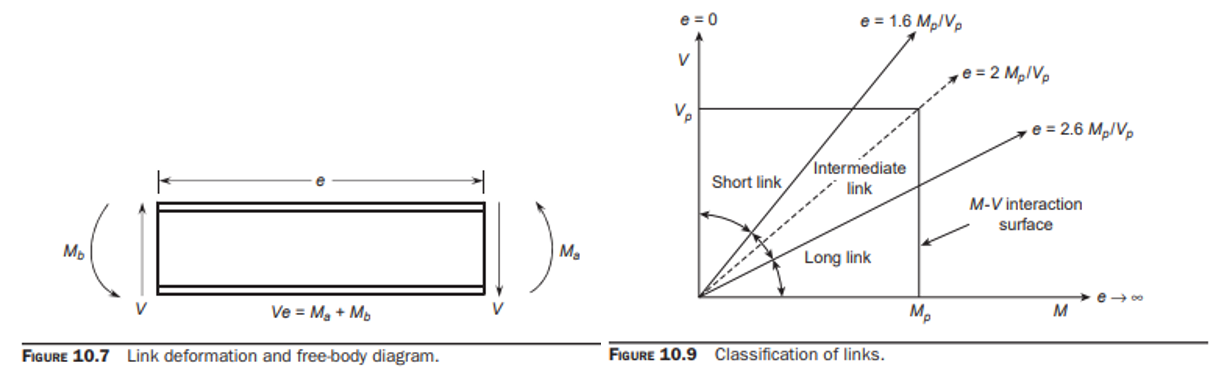
\includegraphics[width=0.9\textwidth]{image99}
	\end{figure}			
	\end{itemize}
\end{block}

	\end{frame}


\note{Test}

	\begin{frame}{3.1 보}

	\textbf{3.1.2 보의 강성}

	3.1.2.1 선형동적절차

선형동적절차를 위한 보의 강성은 구조역학 원칙에 기반하여 $\ulcorner$건축물 강구조 설계기준 (KDS 41 31 00:2019)$\lrcorner$에 따라 산정한다. 
	
3.1.2.2 비선형정적절차

\begin{enumerate}
	\item[(1)] 보 부재의 탄성구간 강성은 3.1.2.1에 따라 산정한다. 
	\item[(2)] 보 부재의 비선형 부재력--변형 모델링은 실험이나 정밀해석을 통해 얻어진 관계를 사용하거나, 그림 1-1과 같은 일반화된 부재력--변형 관계로부터 다음을 따른다. 
	\begin{figure}
		\centering
		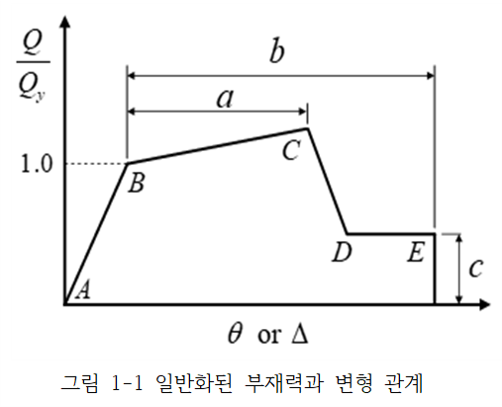
\includegraphics[width=0.5\textwidth]{image01}
	\end{figure}
\end{enumerate}
\end{frame}



\begin{frame}{3.1 보}

	\textbf{3.1.2 보의 강성}

3.1.2.2 비선형정적절차

\begin{enumerate}
	\item[(3)] 보의 길이 $l_b$가 $2.6M_{CE}/V_{CE}$ 이상인 경우 다음을 따른다. 
	\begin{enumerate}[label=\large\protect\textcircled{\small\arabic*}]
		\item 항복회전각 $\theta_y$는 변곡점의 위치를 보 중앙부로 가정하여 다음과 같이 산정할 수 있다. 
		\[\theta_y = \frac{ZF_{ye}l_b(1+\eta)}{6EI_b}\]
		\noindent 여기서 $E$는 탄성계수, $F_{ye}$는 예상재료강도, $I_b$는 보의 단면2차모멘트, $l_b$는 보의 길이, $\eta=12EI_b/(l_b^2GA_s)$, $Z$는 보의 소성단면계수, $A_s$는 유효전단면적, $G$는 전단탄성계수이다. 
		\item 전단변형이 부재 전체 변형의 5\% 이내이거나 해석에 전단에 의한 변형이 포함되지 않은 경우 윗 식의 $\eta$를 0으로 택할 수 있다. 
	\end{enumerate}
\end{enumerate}

	\begin{block}{AISC 342-XX (Draft)}
	Shear deformation (accounted for by $\eta$) in a flexure-controlled beam with a length greater than $10M_{CE}/V_{CE}$ is generally small and can be neglected in Equation C2-2.
\end{block}	

\end{frame}


\begin{frame}{3.1 보}

	\textbf{3.1.2 보의 강성}

3.1.2.2 비선형정적절차

\begin{enumerate}
	\item[(4)] 보의 길이 $l_b$가 $1.6M_{CE}/V_{CE}$ 미만인 경우 보 부재는 전단거동으로 간주하고, 이 때 항복회전각 $\theta_y$는 3.7절에의 식(3.7-2)의 편심거리 $e$에 보의 길이 $l_b$를 대입하여 산정한다. 
\begin{block}{식(3.7-1)과 식(3.7-2): 링크보의 탄성구간 강성과 항복회전각 산정}
	\[K_e = \frac{12EI}{e^3(1 + \eta)},~\theta_y = \frac{Q_{CE}}{K_ee}\]
	\begin{enumerate}
	\item[(1)] 링크보의 예상부재강도 $Q_{CE}$는 예상전단강도 $V_{CE}$ 혹은 예상휨강도 $M_{CE}$에 의해 지배된다(...이하 후술).
	\end{enumerate}
\end{block}	
	\item[(5)] 보의 길이 $l_b$가 $1.6M_{CE}/V_{CE}$ 이상 $2.6M_{CE}/V_{CE}$ 미만인 경우 보 부재는 전단--휨지배거동으로 간주하며, 보의 모델링 변수는 보의 길이에 따라 보--휨과 보--전단에 대해 선형보간하여 산정한다. 
\end{enumerate}
\end{frame}

\begin{frame}{3.1 보}

	\textbf{3.1.2 보의 강성}

3.1.2.3 비선형동적절차

보 부재의 이력거동 모델링은 실험이나 정밀해석을 통해 얻어진 관꼐를 사용할 수 있으며, 포락곡선으로는 표 3-1에 사용된 모델을 적용할 수 있다. 

		\begin{figure}
		\centering
		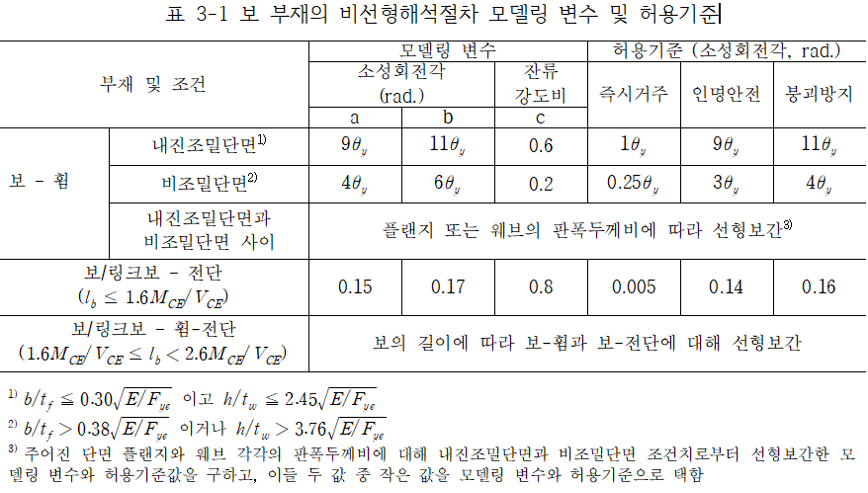
\includegraphics[width=.9\textwidth]{table01}
	\end{figure}
\end{frame}


\begin{frame}{3.1 보}

	\textbf{3.1.3 보의 강도}

3.1.3.1 선형동적절차

\begin{enumerate}
	\item[(1)] 보의 예상부재강도 $Q_{CE}$는 휨항복, 횡좌굴, 플랜지국부좌굴, 웨브전단항복의 한계상태를 고려하여 최솟값으로 산정한다. 
	\item[(2)] 웨브전단항복을 제외한 한계상태에 대해 보의 휨강도는 $\ulcorner$건축물 강구조 설계기준$\lrcorner$에 제시된 공칭강도 $M_n$에 따라 산정하되, 아래의 사항을 고려한다. 
	\begin{enumerate}[label=\large\protect\textcircled{\small\arabic*}]
		\item 변형지배거동이 예상되는 보 부재의 예상휨강도 $M_{CE}$는 강재의 예상재료강도 $F_{ye}$를 적용하여 산정한다. 
%			\[Q_{CE} = M_{CE} = ZF_{ye}\] 소성강도로, 이후의 m계수와 상충
		\item 힘지배거동이 예상되는 보 부재의 하한휨강도 $M_{CL}$은 강재의 최소재료강도를 적용하여 산정한다. 
	\end{enumerate}
	\begin{block}{ASCE 41-17 9.5.3.4 AC for EBF}
Shear and flexure in link beams shall be considered deformation-controlled actions. All other actions, and actions on other EBF somponents, shall be considred force controlled. 
	\end{block}		
\begin{block}{AISC 342-XX (Draft): STRUCTURAL STEEL BRACED BRAME}
	$m=1$ when the beam is classified as a slender section (...) and the top flange is laterally braced at a spacing exceeding limiting laterally braced length for the limit state of inelastic LTB.
\end{block}	
	\item[(3)] 웨브전단항복의 경우 $M_{CE}$는 $V_{CE}l_b/2$로 산정하며 이 때 $V_{CE}$는 3.7절 링크보요소에 따라 산정한다.  
%		\item[(4)] 보의 전단강도 $V_{CE}$는 $\ulcorner$건축물 강구조 설계기준$\lrcorner$에 따라 산정한다. 불필요해보임
\end{enumerate}
\end{frame}	


\begin{frame}{3.1 보}

	\textbf{3.1.3 보의 강도}

3.1.3.2 비선형정적 및 동적절차

\begin{enumerate}
	\item[(1)] 비선형정적절차의 경우 표 3-1에 따라 그림 1-1과 같은 비선형 부재력--변형 관계를 결정한다. 보의 예상부재강도 $Q_{CE}$는 선형절차와 동일한 값을 사용한다. 
	\item[(2)] 비선형동적절차의 이력거동 모델링은 실험이나 정밀해석을 통해 얻어진 관계를 사용할 수 있으며, 포락곡선으로는 표 3-1에 사용된 모델을 적용할 수 있다. 
\end{enumerate}
\end{frame}	


	\begin{frame}{3.1 보}

	\textbf{3.1.4 보의 허용기준}

3.2.4.1 선형동적절차

\begin{enumerate}
	\item[(1)] 선형동적절차를 위한 보의 허용기준은 표 3-2를 따른다. 
	\item[(2)] 횡비틀림좌굴로 인해 예상휨강도가 $M_{pe}$보다 작은 경우, 부재별 허용기준은 표 3-2에 의한 $m$대신 다음의 $m_e$를 사용하여 판정한다. 
	\[m_e = m - (m - 1)\frac{M_{pe} - M_{CE}}{M_{pe} - (0.7F_{ye})S} \geq 1.0\]
	\noindent 여기서 $M_{pe}$는 강축에 대한 예상소성휨강도, $M_{CE}$는 예상모멘트, $S$는 보의 탄성단면계수, $m$은 $m$계수이고, $m_e$는 수정$m$계수이다. 
\end{enumerate}

3.2.4.2 비선형 정적 및 동적절차	

보 부재의 소성회전변형 허용기준은 표 3-1을 따른다. 
\end{frame}	

	\begin{frame}
	\begin{figure}
		\centering
		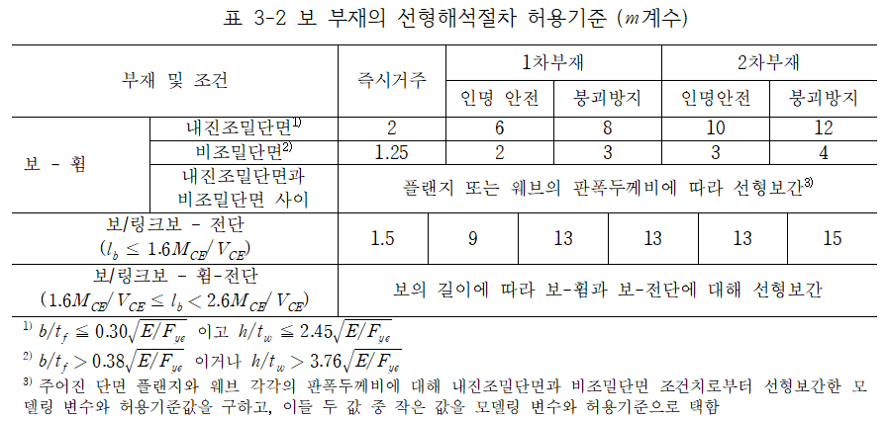
\includegraphics[width=.99\textwidth]{table02}
	\end{figure}
\end{frame}	
